\section{Обзор литературы}
Задача автоматизированного выявления паттернов в бинарных программах известна достаточно давно (одной из первых работ в этой области является \cite{bugs}). Существующие способы решения используют в основном статический и динамический анализ, основанный на различных эвристиках. Но сравнительно недавно стали очень активно развиваться методы анализа, основанные на машинном обучении. В этом разделе рассматриваются несколько существующих на данный момент подходов по распознаванию семантики исходного кода с анализом их плюсов и минусов в контексте применения для выявления паттернов в скомпилированных бинарных программах.

\subsection{Graph2Seq}
В данной статье\cite{xu2018graph2seq} авторы представляют модель типа кодер-декодер для перевода входных данных в виде графа в последовательность. Сначала к графу применяются сверточные слои с нелинейными активациями, затем с помощью операции пуллинга всех векторных представлений получается векторное представление графа. Полученное векторное представление передается на вход рекуррентной нейронной сети с механизмом внимания. Авторы получили лучшие или близкие к лучшим результаты для 3 задач: первые две относились к поиску кратчайшего пути в графе, последняя к переводу запросов языка SQL в описание на естественном языке. Ниже представлена схема, описывающая работу данной модели:
\begin{figure}[h]
    \center{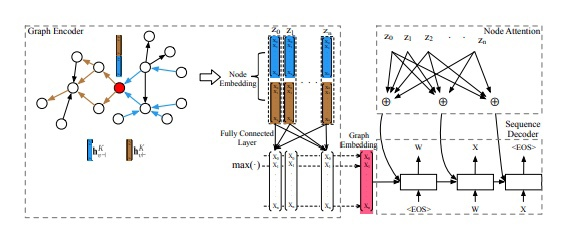
\includegraphics[width=0.9\linewidth]{images/GRAPH2SEQ.jpg}}
    \caption{Схема модели graph2seq}
\end{figure}

Эта модель может быть с небольшими изменениями адаптирована для задачи graph2vec, например, если совсем убрать декодер, или полученную последовательность подать на вход модели seq2vec. При этом во втором случае элементы последовательности будут содержать информацию о всем графе, и каждый элемент последовательности сильнее учитывает значение соответствующей вершины в исходном графе.

\subsection{Improved Code Summarization via a Graph Neural Network}
В работе\cite{leclair2020improved} авторы решали задачу суммаризации кода, основываясь на работе graph2seq. Модель представляет собой кодер-декодер с несколькими входами. Модель последовательно предсказывает текст-описание функции, на каждой итерации получает на вход последовательность токенов кода, его абстрактное синтаксическое дерево и предсказанную до текущего момента последовательность. Затем токены переводятся в соответствующие векторные представления и подаются на вход GRU. Абстрактное синтаксическое дерево с соответствующими векторными представлениями проходят 2 сверточных слоя и подаются на вход GRU. Предсказанная к текущему моменту последовательность переводится в векторные представления и подается на вход GRU. Далее полученные последовательности соответствующие абстрактному синтаксическому дереву и предсказанной последовательности передаются в механизм внимания. Аналогично обстоит дело с последовательностью, соответствующей исходным токенам. Затем полученные векторы объединятся, подаются в линейный слой. Полученный вектор можно использовать для предсказания следующего токена.
\begin{figure}[h]
    \center{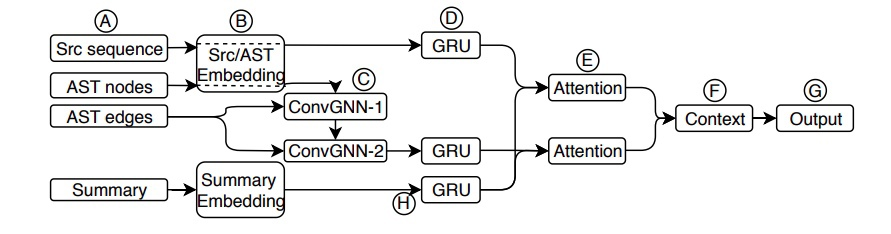
\includegraphics[width=0.9\linewidth]{images/gnn1.jpg}}
    \caption{Модель использующая GCN для суммаризации}
\end{figure}

\subsection{Retrieval-Augmented Generation for Code Summarization via Hybrid GNN}
В работе\cite{liu2021retrievalaugmented} авторы также решали задачу суммаризации кода. Модель представляет собой кодер-декодер. Модель работает следующим образом:
\begin{itemize}
    \item По имеющемуся исходному коду строится CPG граф\cite{6956589}, последовательность признаков вершины и ее тип кодируются с помощью матриц векторных представлений. Преобразованная последовательность признаков подается в двунаправленный LSTM блок;
    \item
        \begin{itemize}
            \item Ищется наиболее похожий код в имеющемся обучающем наборе данных;
            \item Вычисляется матрица внимания на основе всех векторных представлений вершин найденного кода и исходного; Полученная матрица умножается на коэффициент схожести найденного кода и матрицу векторных представлений найденного кода. Эта матрица прибавляется к матрице исходного кода;
            \item Описание для найденного кода кодируется с помощью векторных представлений и подается в двунаправленный LSTM блок. Позже выход LSTM умножается на коэффициент близости, конкатенируется с выходом GNN и подается в декодер.
        \end{itemize}
    \item Строится динамический граф (точнее, его матрица смежности) на основе механизма внимания, чтобы была возможность передачи информации между двумя произвольными вершинами. Затем нормализуется;
    \item Вычисляются векторы агрегированные векторы после свертки на статическом и динамическом графах, вычисляется взвешенная сумма с вычисляемыми коэффициентами и подается на вход GRU блоку;
    \item Декодер представляет из себя LSTM и получает на вход векторы из GRU и поданного в LSTM блок описания для ближайшего найденного кода.
\end{itemize}

\begin{figure}[h]
    \center{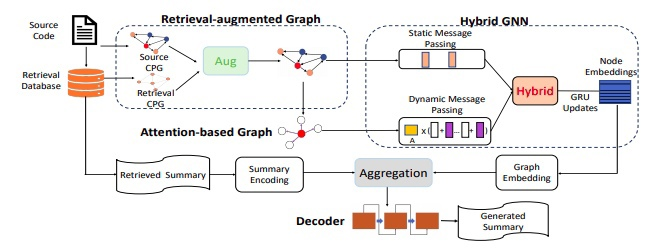
\includegraphics[width=0.8\linewidth]{images/HGNN.jpg}}
    \caption{Hybrid GNN}
\end{figure}

\subsection{Inst2vec}
Используя метод inst2vec\cite{ncc} авторы предложили решение сразу 3 задач. Первая задача состояла в определении класса алгоритма. Во второй задаче надо было определить, на каком вычислительном устройстве (центральный процессор или видеокарта) выгоднее запустить программу, чтобы ее время исполнения было меньше. Третья задача заключалась в определении максимального количества нитей при запуске кода на видеокарте для минимизации времени работы. Для решения этих задач использовался подход с обучением векторного представления инструкций.

Т.к. исходный код для этих задач может быть написан на разных высокоуровневых языках, то с целью генерализации подхода авторы выбрали представление llvm ir, в которое может быть скомпилирован код на большом множестве языков, например, на C/C++, FORTRAN, Python, Java, CUDA, OpenCL и др. Было сделано предположение, что инструкции, которые находятся "близко" друг к другу, имеют похожий смысл. Поэтому для обучения векторных представлений были выбраны модели Word2vec\cite{DBLP:journals/corr/MikolovSCCD13} и Skip-Gram, использование которых предполагает наличие понятия контекста слова(в данном случае инструкции).

Авторы определяют контекст инструкции, как множество инструкций, от которых напрямую зависит выполнение данной инструкции. Таким образом учитывается зависимость как по передаче управления, так и зависимость по данным. Инструкции с вышеупомянутой зависимостью не могут быть напрямую извлечены из исходного кода, поэтому сначала строится XFG (contextual-flow graph) граф. Это ориентированный мультиграф, который определяется следующим образом: вершинами являются переменные или метки, например, базовые блоки, функции; ребра являются либо зависимостью по данным либо зависимостью по управлению; если у инструкции нет зависимости по данным, она соединяется ребром с корневой вершиной. Для того, чтобы словарь не был очень большим данные подвергались предобработке. Убирались комментарии и метаданные, константы заменялись на фиксированные токены, имена переменных заменялись на специальный токен, производилась подстановка структур.

После обучения векторных представлений для решения поставленных задач обучалась рекуррентная нейронная сеть, которая принимала на вход преобразованную в векторное представление последовательность инструкций llvm ir (рисунок \ref{ris:inst2vec}).
\begin{figure}[h]
    \center{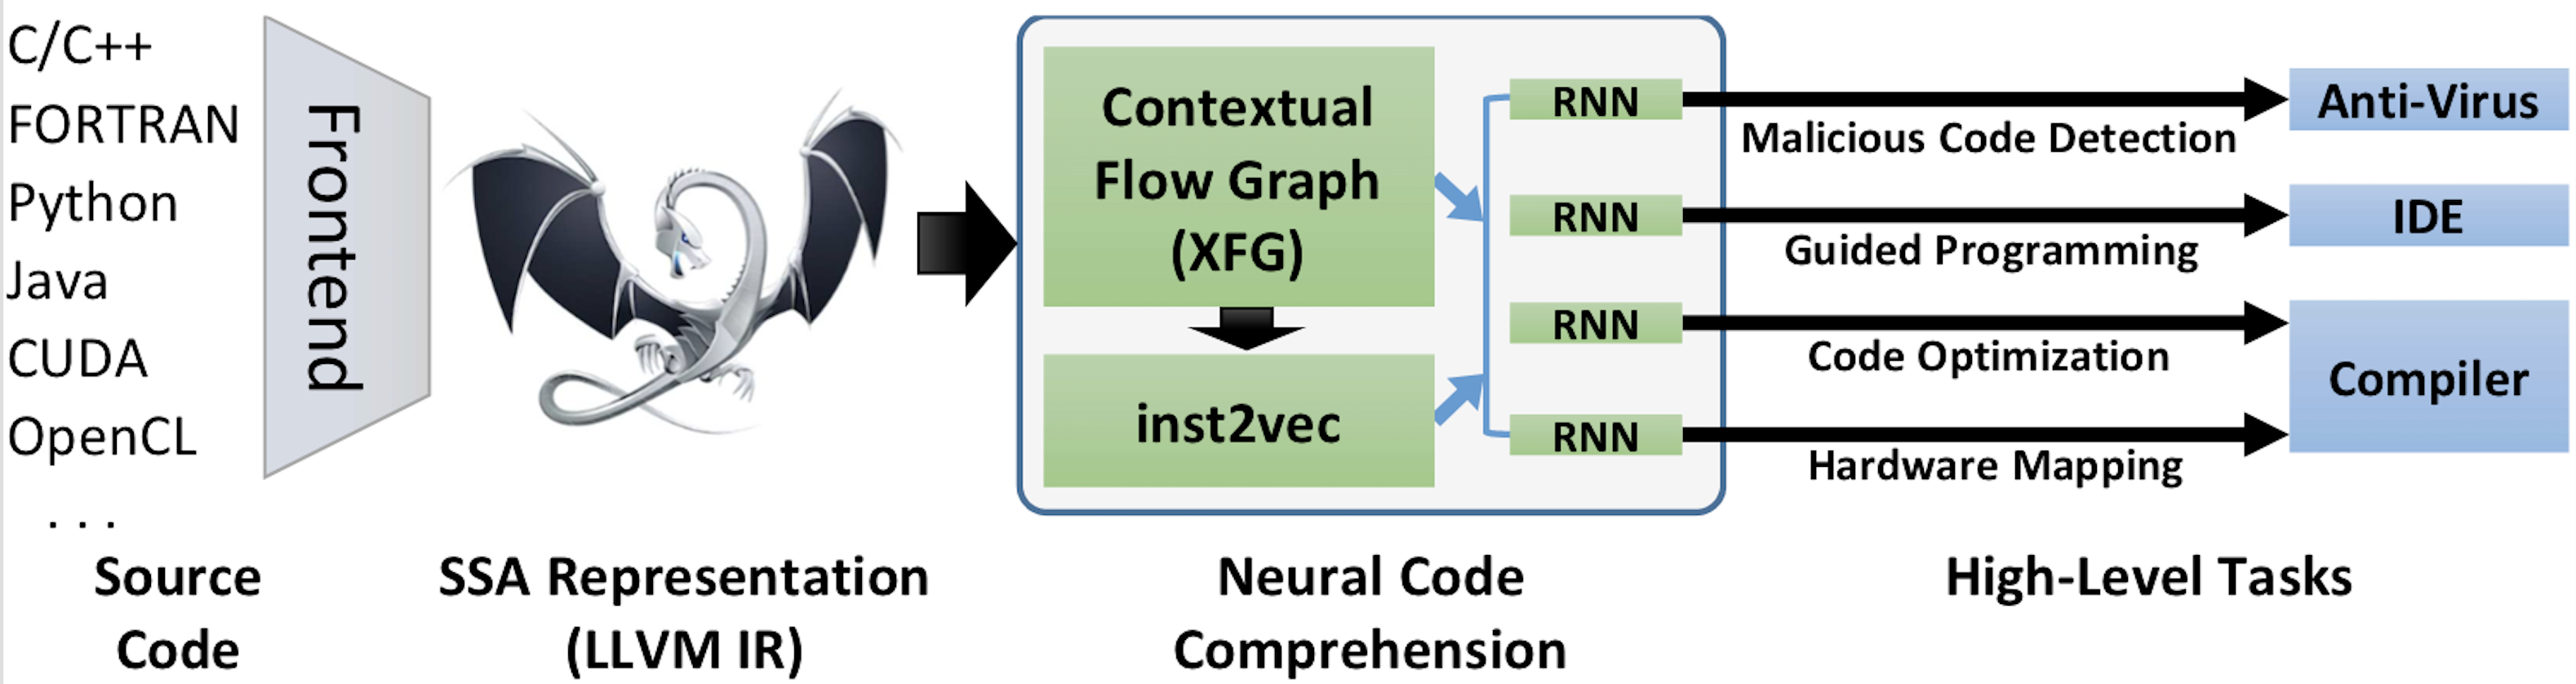
\includegraphics[width=0.9\linewidth]{images/inst2vec.jpg}}
    \caption{Принципиальная схема модели inst2vec}
    \label{ris:inst2vec}
\end{figure}

Данный подход имеет свои плюсы, важнейшими из которых является обобщённость и возможность повторного использования векторных представлений. Также стоит отметить, что этот подход является наиболее простым с вычислительной точки зрения, относительно других подходов, рассмотренных ранее. 